\section{Introduction}
This Chapter deals with realising and validating an experimental set-up to measure the temperature dependent surface photovoltage (\spv{}(T)) with the help of a cryogenic system, a modified Kelvin probe (\kp{}) and a suitable source of illumination. Section \ref{sec:theo} will introduce the necessary physical background underlying the measurements with a \kp{} and will be followed by a more thorough description of the actual Kelvin probes in use in Section \ref{sec:kp}, subdivided into a description of the already established systems (Section \ref{sec:kppold}) and the \enhyphen{new} system (Section \ref{sec:kpnew}). The experimental approach described in the following Sections is aimed at validating, step-by-step that the \enhyphen{new} system reproduces results obtained with the established systems and to investigate possible complications that the capabilities of the \enhyphen{new} system might bring to light. The experimental approach will culminate in a report of a temperature dependent measurement of the \spv{} for a chosen model system in Section \ref{sec:vox}. While results obtained in that last Section cannot be fully explained at this point, the measurement did serve as a useful proof of principle to show that reproducible \spv{}(T) measurement are feasible with the system. A brief conclusion will round off this Chapter.

\section{Theory}
\label{sec:theo}
\subsection{The Contact Potential Difference and the Kelvin Probe}
When two (semi-)conductors with dissimilar Fermi levels are electrically connected from their back-side with a gap between them, charge will flow from the material with the lower work function (\wf{}) to the one with the higher \wf{}. The work function is defined as the energy needed to remove an electron from a solid to a point in vacuum immediately outside of it. Electrons will stop flowing when equilibrium is established. As long as there is a gap between the materials, an electrical field will develop in the gap due to the difference in the local vacuum level across this gap. 
The potential drop across the gap, the contact potential difference or \cpd{}. When the work functions are expressed in Electron-Volts, the \cpd{} is directly equal to the difference of the \wf{}s:
\begin{equation}
\label{wf}
	{\cpd} \, \equiv \,  \wfp \, - \wfs \, .
\end{equation}
The order of the operands in the equation above is a matter of convention. Their physical representation depends on how the measurement system which we will investigate in the following -- the Kelvin Probe -- is set up electrically. 
In the configuration outline above, the materials behave like a parallel plate capacitor and a capacitance is established, which is known to be:
\begin{equation}
\label{cap}
	C(t) = \frac{\epsilon \epsilon_0 A}{d(t)} \,
\end{equation}  
in which $\epsilon$ \& $\epsilon_0$ are the permittivity and the permittivity of free-space respectively, $A$ is the area of the parallel plate and $d(t)$ is the distance between the plates. $d(t)$ is taken as a function of time, because the Kelvin Probe varies the distance in time. The current between the plates is given by the change in charge on the plates, which is in turn given by the change in capacitance:
\begin{equation}
	I(t) = \frac{dQ}{dt}= \Delta V \frac{dC}{dV} \, ,
\end{equation}
where $\Delta V$ is the difference in potential between the plates, which is the sum of the applied backing voltage and the naturally occurring potential difference between the plates, the \cpd{}: $\Delta V = V_{\text{Backing}} + \cpd$. If we assume a sinusoidally varying distance with the average distance between the plates being $d_0$, $d_1$ being the amplitude of oscillation, $\omega$ being its frequency of oscillation and an arbitrary phase $\psi$, then
\begin{equation}
	d(t) = d_0 + d_1 \sin (\omega t + \psi)\, 
\end{equation}
and finally
\begin{equation}
\label{current}
	I(t,\Delta V) = -\epsilon \epsilon _0 A \Delta V \frac{d_1 \omega \cos (\omega t + \psi}{(d_0 + d_1 \sin (\omega t + \psi))^2}\, .
\end{equation}
In equation \eqref{current}, the current is written as a function of time and potential difference between the plates, because while continuously varying the distance between probe and sample, the Kelvin Probe also varies $V_{\text{Backing}}$. As can easily be seen from equation \eqref{current}, the current is zero or 'nulled' when $V_{\text{Backing}}=-\cpd$. Thus, if \wfp{} is known, \wfs{} can easily be calculated from equation \eqref{wf}. In practice, this requires calibrating the probe head against a sample with known work function, \hopg{} in the context of this study. Obviously, if one wants to study the work function of a sample as a function of temperature, the temperature dependence of the work function of the probe also has to be known. In most cases and especially for simple metals, the work function only varies over a few hundredths to a few tenths of meVs per Kelvin~\cite{tempdepmet,tempdepmet2,tempdepmet3,tempdepmet4,tempdepmet5}. These variations are negligible compared to other sources of experimental uncertainty and the work function of the probe is therefore assumed to be constant with respect to temperature throughout this work.\\
As pointed out, the work function \wf{} of a semiconductor is defined as the the energy needed to remove an electron from the material to a point in vacuum just outside of it and is given by the difference of the near surface vacuum vacuum energy $E_{\text{vac}}$ and the Fermi energy $E_{\text{f}}$ of the material: $\upvarphi = E_{\text{vac}} - E_{\text{f}}$. The Fermi level of a doped semiconductor is dependent on the temperature and the carrier-concentrations of the semiconductor and can be expressed in terms of the intrinsic Fermi energy as:\\[5pt]
\begin{minipage}[c]{0.4\textwidth}
	\begin{equation}
	\label{efn}
	E_{f,n} \, =  E_i \, - \, kT \ln{\frac{n}{n_i}}
	\end{equation}
\end{minipage}	
\hfill
and
\hfill
\begin{minipage}[c]{0.4\textwidth}
	\begin{equation}
	\label{efp}
	E_{f,p} \, = E_i \, + \, kT \ln{\frac{p}{p_i}}
	\end{equation}
\end{minipage}\\[5pt]
for n- and p-type semiconductors respectively. As can be seen from the preceding equations, $E_{f}$ changes with the Boltzmann Temperature. At 300 K~\footnote{approximately room temperature} and at 100 K, $kT$ is approximately equal to 26 and 8.6 meV, respectively. In many cases, it is assumed that the extrinsic carrier concentrations $n$ and $p$ are equal to the product of dopant concentration and number of supplied free carriers per dopant atom. But even in that case, the concentration of intrinsic carriers is still a strong function of temperature and requires knowledge of several material parameters to calculate precisely. A simpler argument that is valid for moderately doped semiconductors in which the Fermi-Dirac distribution can be approximated by the Boltzmann distribution is developed in the following for the example of an n-type semiconductor. In such a semiconductor, the chance of finding an electron close to the conduction band edge is greater than finding a hole close to the valence band edge. Therefore, the Fermi level is closer to the conduction band. At absolute zero, all levels below the Fermi level are filled and all levels above the Fermi level are empty, by definition. At absolute zero, there can be no free electrons as freedom to move would imply energy. Therefore, at absolute zero, the Fermi level cannot be above the conduction band edge. So far, it is shown that the Fermi level must be closer to the conduction band, but below its band edge. At extremely high temperatures, doping will be negligible because thermally generated carriers will exceed carriers introduced by the dopant. Therefore, the Fermi level will tend toward the intrinsic Fermi level in mid gap. A similar argument holds for the Fermi level of a moderately doped p-type semiconductor and it is therefore shown that:\\[5pt]
\begin{minipage}[c]{0.4\textwidth}
	\begin{equation}
	\frac{dE_{f,n}}{dT} < 0
	\end{equation}
\end{minipage}	
\hfill
and
\hfill
\begin{minipage}[c]{0.4\textwidth}
	\begin{equation}
	\frac{dE_{f,p}}{dT} > 0
	\end{equation}
\end{minipage}\\[10pt]
for the Fermi level of an n-type and a p-type semiconductor, respectively.
\subsection{The Surface Photovoltage and Band Bending}
In the context of this work, the surface photovoltage (\spv{}) is defined as the \cpd{} measured under illumination minus the \cpd{} in the dark:
\begin{equation}
\label{spv}
	\spv \equiv \cpd_{\text{light}} - \cpd_{\text{dark}} \, .
\end{equation}
\begin{figure}
\begin{subfigure}{0.5\textwidth}
\centering
	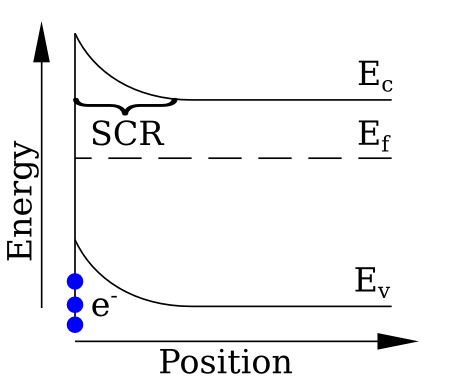
\includegraphics[width=0.8\linewidth]{./figs/chap2/bb-dark}
	\caption{}
	\label{fig:bbdark}
\end{subfigure}
\begin{subfigure}{0.5\textwidth}
\centering
	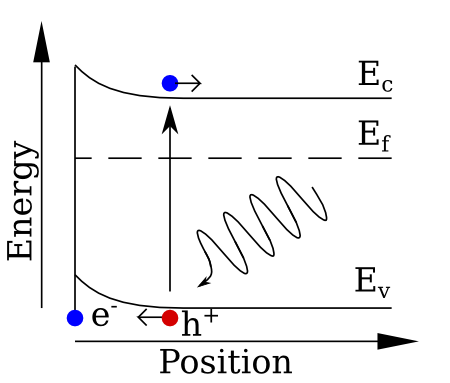
\includegraphics[width=0.8\linewidth]{./figs/chap2/bb-light}
	\caption{}
	\label{fig:bblight}
\end{subfigure}
\caption{Band bending, trapped surface charges and the space charge region at the surface of an n-type semiconductor (a) in the dark and (b) under illumination. Note the decrease in trapped surface charges in (b) and the resulting reduction in band bending. Energy levels of the valence band, $E_v$, the Fermi level, $E_f$, and the conduction band, $E_c$, are included for reference.}
\label{fig:bb}
\end{figure}
It is instructive to refer to the diagrams in Figure \ref{fig:bb} to understand the origin of the surface photovoltage: in the dark, majority carriers are trapped at the surface, setting up a space charge region (\src{}). For n-type semiconductors, electrons are in the majority, accumulating negative charge on the surface, setting up an electrical field pointing from the bulk toward the surface. This field causes the potential energy of electrons to be higher at the surface than in the bulk and accordingly, the bands in Figure \ref{fig:bbdark} are bent 'up'. Of course, the situation is reversed for p-type semiconductors. Under illumination, electron-hole pairs are created where radiation of sufficient energy is absorbed. For direct band-gap semiconductors, the absorption depth is shallow and electron-hole pair generation might well occur within the \src{}. For indirect band-gap materials, absorption might occur deep within the bulk and carriers might have to diffuse through the material until they reach the \src{}. Regardless of their path, once the carriers are close to or within the \src{} the direction of the electrical field present there causes minority carriers to be attracted to the surface and majority carriers to be repulsed back to the bulk. Once the minority carriers reach the surface, they will recombine with majority carriers already present there. This causes the charge at the surface to decrease and the bands to flatten, see Figure \ref{fig:bblight}. When the trapped surface charge is completely neutralised, the bands will return to their initial flat state, the \src{} will vanish and it is said that the \spv{} has saturated~\cite{yates_bandbend}. Saturation is usually assumed in an experiment when a further increase in illumination intensity does not lead to a further change in observed light \cpd{}. For this reason, \spv{} is often the method of choice when investigating the band bending~\cite{macnamara_tempdepspv,macnamara_tempdepspv2} but it should be noted that in the presence of strong Fermi level pinning, bands might still be bent, even if \spv{} saturation is reached~\cite{kronik_spv}. In that case, bending is not exclusively due to trapped charges and care should be taken when analysing results obtained by \spv{}. In a metal, the Fermi level lies within the conduction band. Therefore, carriers are free to move to and from the surface and no notable \src{} will exist in a metal. Therefore, no difference in \cpd{} between the dark and the illuminated condition is expected for a metal, so equations \eqref{wf} and \eqref{spv} combine to give the \spv{} as a function exclusively in terms of the sample material:
\begin{equation}
\label{spvs}
	\spv = \upvarphi _{\text{s,dark}} - \upvarphi _{\text{s,light}} \, .
\end{equation}
To gain a deeper insight into the behaviour of a semiconductor as it reacts to light, its work function can be redefined in more practical terms, namely in terms of electron affinity, band-bending, conduction band edge and Fermi level, which are shown in Figure \ref{fig:terms}. 
\begin{figure}
\begin{subfigure}{0.5\textwidth}
\centering
	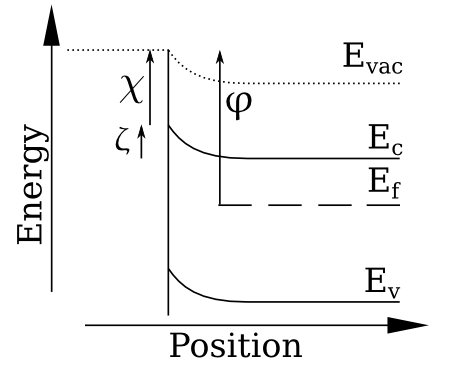
\includegraphics[width=0.8\linewidth]{./figs/chap2/bbdefn-2}
	\caption{}
	\label{fig:bbdefn}
\end{subfigure}
\begin{subfigure}{0.5\textwidth}
\centering
	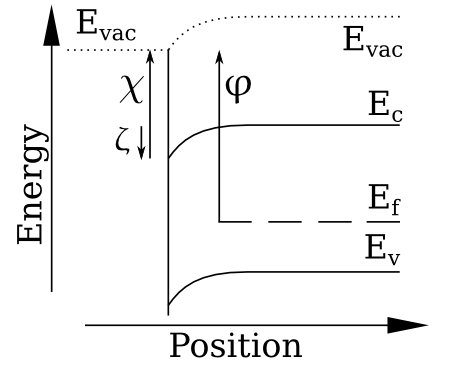
\includegraphics[width=0.8\linewidth]{./figs/chap2/bbdefp-2}
	\caption{}
	\label{fig:bbdefp}
\end{subfigure}
\caption{Definition of terms electron affinity, $\chi$, band-bending $\upzeta$, conduction band edge, $E_c$, Fermi level, $E_f$ and work function, $\upvarphi$, for an n-type semiconductor (a) and a p-type semiconductor (b). It can be shown that the band bending is negative for the p-type semiconductor. Valence band edge, $E_v$, included for reference.}
\label{fig:terms}
\end{figure}
The electron affinity is the energy gained by moving an electron from the conduction band at the surface to a point in vacuum just outside the solid:
\begin{equation}
\label{Eea}
	\chi \equiv E_{\text{vac}} - E_c \, .
\end{equation}
Band-bending, $\upzeta$, is defined as the energy difference between the conduction band at the surface and the conduction band deep inside the semiconductor. Using these terms, the work function is then obtained as:
\begin{align}
\label{wfbb}
	\upvarphi &\equiv E_{\text{vac}} - E_f \\
	 &= E_c + \chi + \upzeta - E_f \, .
\end{align}
In the equation above, $\chi$ and $E_c$ are not affected by illumination, band-banding vanishes under saturation~\footnote{in the absence of Fermi level pinning} and $E_f$ can change because of its dependence on the carrier concentrations as expressed in equations \eqref{efn} and \eqref{efp}. Combining equations \eqref{wfbb} and \eqref{spvs} yields an interesting property of the \spv{}: its sign can be used to identify if a sample is n- or p-type. For both n- and p-type semiconductors, the absolute value of $\upzeta$ is larger in the dark than under illumination. For an n-type semiconductor, $\upzeta$ is positive and thus its \spv{} is also a positive quantity; for a p-type semiconductor, the situation is reversed: both $\upzeta$ and \spv{} are negative, thus:
\begin{align}
	\spv 	&= \upvarphi _{\text{s,dark}} - \upvarphi _{\text{s,light}} \\
			&= \upzeta _{\text{dark}} - \upzeta _{\text{light}} + E_{f\text{,light}} - E_{f\text{,dark}} \, ,
\end{align}
where the difference in Fermi levels can be assumed to be small and where $\upzeta _{\text{light}}$ tends to zero under saturation and in the absence of Fermi level pinning.

\section{Kelvin Probes in Use}
\label{sec:kp}
\subsection{Established Kelvin Probe System}
\label{sec:kppold}
As mentioned, it was the aim of this project to establish if a combination of a cryogenic system fitted with a custom \kp{} probe head could be used for temperate dependent measurements of the \spv{}. The system in question will be described in detail in Section \ref{sec:kpnew}, here, the focus will be on a brief description of the two Kelvin probe system that were already established and had been in use in the Cahen group for some time.\\
Both systems feature \kp{} probe heads model \enhyphen{Kelvin Probe S}, manufactured by Besocke Delta Phi GmbH~\cite{besocke}, electrical and mechanical control is provided by systems provided by the same manufacturer. Housing and illumination for the Kelvin probe set-ups are provided by in-house built solutions. The probe head consists of a \SI{2.5}{\milli\metre} diameter opaque gold grid and as such provides a stable and inert reference surface for measurements of the \cpd{}. In practice, however, the probe heads still need to be calibrated with \hopg{} if absolute measurements of the \wf{} are desired because changes in humidity, contamination or other, unknown factors can greatly influence the work function of the probe heads.\\
The first Kelvin probe system is situated in a shielding Faraday cage placed inside a humidity controlled room (\SI{20}{\percent} relative humidity) and the probe head is exposed to ambient. This system will be referred to as the \enhyphen{Ambient Probe Station}. The sample is mounted onto a conductive block of metal which is slid into a holder that provides an electrical ground for the sample specimen. Samples are either connected with InGa eutectic via their backside or with the help of an electrically conductive clip-holder screwed to the conductive block of metal. The sample is stationary and the probe head is positioned close to the surface under investigation with the help of micrometer screw gauges. Illumination of the sample is achieved with a xenon-lamp driven by a VariAC-power source with up to \SI{60}{\watt} electrical power and an optical lens focusing the light onto the surface of the mounted sample. The illumination level is controlled manually and increased until saturation of the \spv{} signal is reached. \cpd{} data are collected with a custom LabView program and monitored in real time.\\
The second system is very similar, but is placed inside a humidity and oxygen controlled glovebox (ideally $<\num{5}$ppm \oxy{} \& \water{}) and will therefore be referred to \enhyphen{Glovebox Probe Station} or \enhyphen{Glovebox 301}~\footnote{The glovebox and its probe station are situated in room 301 on a different floor than the other experimental facilities of the Cahen group.}. Mounting and electrical connection of the sample are virtually identical to the Ambient Probe Station, but illumination offers more flexibility. On the one hand, an identical illumination set-up, also using a xenon-lamp and VariAC source can be used. On the other, the system is fitted with a more advanced illumination scheme to allow for Surface Photovoltage Spectroscopy (\sps{}) measurements over a spectral range spanning \ir{} to ultraviolet (\uv{}) radiation. These capabilities were not use in this project and so shall not be further described. For the purposes of this project, the Ambient and Glovebox probe stations are practically identical and offer a trusted source of comparison for \cpd{} and \spv{} data taken with the new, to be developed system. Influences of the atmosphere, viz. clean nitrogen vs. ambient, were investigated but were found to be negligible compared to the unavoidable experimental uncertainties in \cpd{} and \spv{} measurements.
\subsection{The Lakeshore Cryogenic System coupled with a \McA{} Kelvin Probe}
\label{sec:kpnew}
Lakeshore is an international vendor of cryogenic probe stations. For this research, a Lakeshore Model TTPX Probe Station was used. The probe station can be thought of as being divided into four components. An outer vacuum-chamber is connected to a pump to reduce the pressure inside the station. An Argon gas inlet connected to the vacuum chamber can be used to provide an inert atmosphere. Inside the vacuum chamber is a separate, smaller chamber: the radiation shielding stage, primarily used to shield the sample from \ir{} radiation and thus used to facilitate measurements at low temperatures. The radiation shielding to some extend also provides electrical shielding from stray electrical signals and can therefore act as a quasi Faraday-cage. Both these chambers are fitted with windows to allow for placement of the probe-arms and to allow for visual inspection of the experiment. The radiation shielding stage's windows is made from sapphire glass, as sapphire glass is oblique to infra-red radiation. Inside the shielding stage is placed the sample stage, which allows for mounting of samples and can provide an electrical ground. The fourth and last component of the probe station are its six probe-arms. They allow for placement of several probes on the sample from the outside. For many measurements, these probes are conceptually simple gold wires which allow for electrical measurements of the sample, such as IV and CV characterisation. Being a cryogenic system, the Lakeshore is fitted with three thermocouples. They measure the temperature of the sample stage, the radiation chamber and the probe-arm respectively. The temperature is adjusted by an electrical heater and by controlling the flow of of coolant, either liquid nitrogen or -- to achieve lower temperatures -- liquid helium. Evacuation of the cryogenic system is achieved by a combination of two pumps: a `weak pump' to reduce the pressure to $\sim$\SI{5e-2}{\milli\bar} and a \enhyphen{turbo pump} to reduce it down to $\sim$\SI{5e-4}{\milli\bar}. A schematic of the Lakeshore model TTPX cryogenic system showing its components is given in Figure \ref{fig:McAscheme}.\\
\begin{figure}
\centering
	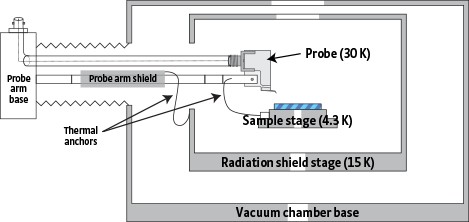
\includegraphics[width=0.8\linewidth]{./figs/chap2/Config_TTPX}
	\caption[Schematic of the Lakeshore model TTPX cryogenic system and its components, typical operational temperatures are indicated.]{Schematic of the Lakeshore model TTPX cryogenic system and its components, typical operational temperatures are indicated. Taken from the vendor's website~\cite{lakeshore}.}
	\label{fig:McAscheme}
\end{figure}
In our case, one of the probe arms is fitted with a modified \McA{} ultra-high vacuum (\uhv{}) Kelvin probe head. The original \McA{} \uhv{} Kelvin probe head is a horizontal base-arm ending in a vibrating, stainless steel cylinder of 2.6 mm diameter ending in a continuous, flat disk. This disk forms one of the two capacitor plates necessary for a \cpd{} measurement. The other capacitor is, of course, the sample. Using the \McA{}, the measured signal is given by equation \eqref{wf} i.e. the signal is equal to the work function of the probe head, usually $\sim$ \SI{4.5}{\electronvolt}, minus the work function of the sample. A reduction in measured \cpd{} therefore means an increase in the sample's work function.\\
The original probe head configuration is not suitable for the Lakeshore cryogenic system because the sample needs to be placed horizontally onto the sample-stage. Therefore, a vertical geometry is needed for the probe-head. Such a custom system was provided by \McA{}. The stainless-steel Kelvin probe head is now vertically mounted in a plastic base. The size and especially the weight-distribution of the original cylinder are carefully designed by \McA{} to comply with a vibration-response that is suitable for the probe head controller. The probe head is electrically connected by a gold wire that runs along the base-arm and is either soldered directly onto the cylinder or tightly wrapped around a conductive screw which is used to hold the probe head in place in its plastic holder. In the latter case, conductive silver paste suitable for \uhv{} environments is applied to the screw to ensure low resistance electrical connection. Contact potential difference measurements are severely negatively affected by non-ohmic back contacts. A second probe arm of the cryogenic system was fitted with an optical fibre to allow for laser illumination of the sample. However, in practice, it quickly became clear that such an illumination set-up was unsuitable for \spv{} measurements. This was due to several reasons. For suitable \cpd{} measurements, the probe head needs to be brought in very close proximity to the sample: distances on the scale of a few hundred micrometers are often necessary to obtain a sufficiently noise-free signal~\footnote{This adds to the practical danger of involuntarily crashing the vibrating probe head onto the sample, potentially damaging the sample, contaminating the probe head and generally interfering with conducting an experiment}. Therefore, there is simply not enough room for the exit of the optical fibre to be placed in a position where light would illuminate the sample. A further difficulty of the fibre illumination scheme are noticeable reductions in light intensity due to absorption in the fibre. After all, the fibre needs to be able withstand vacuum conditions and low temperatures, limiting the choice of suitable materials. Lastly, the fibre would provide a very localised spot of illumination. For a successful measurement of the \spv{}, the whole area under the probe head has to be saturated by illumination at the very least. Full saturation of the whole sample surface is in most cases desirable to suppress unwanted carrier recombination in the dark areas. For these reasons, it was decided to modify the probe head and employ a different illumination scheme. The cryogenic system's windows allow for illumination by a source of light placed outside the vacuum chamber, on top of the external window, focused onto the sample surface. To allow this scheme to work, the main body of the probe head needed to be hollowed out and holes needed to be drilled into the head's disk to let light pass through and onto the sample. Such a probe head, manufactured from stainless steel, was provided by \McA{} and used in initial experiments. When successful measurements were not forthcoming, three further modifications of the probe head were tried, all based on the same principle. The idea was to replace the massive disk with a wire-grid used for transmission electron microscopy (\tem{}). Three different types of wire-grids were purchased from Structure Probe Inc., a stiff, stainless steel grid with \SI{70}{\percent} opacity, two thin, flexible gold grids with \SIlist{70;60}{\percent} opacity respectively. The grids were laser-welded onto custom-made, hollowed out stainless steel cylinders. These new probe heads were manufactured by the Weizmann Institute's Department for Construction and Engineering. Care was taken to ensure acoustic vibration characteristics of the new probe heads were similar, if not identical to those of the original \McA{} probe heads. The wire-grids would add two benefits: they would increase the overall transmission of the probe head as well as allow for a more even illumination of the sample surface. In practice, however, no immediate, significant difference between the performance of the original hollow stainless steel probe head and the new, \tem{} wire-grid heads was found. At this point, an inherent limitation of the adopted illumination scheme has to be pointed out: namely that even in the ideal case, illumination from above will only result in an illuminated area directly under the probe head. The probe arm, probe head holder and even the edge of the hollow cylinder will all cast a a shadow on the sample, especially since they need to be placed directly above it.\\
\begin{figure}
\centering
	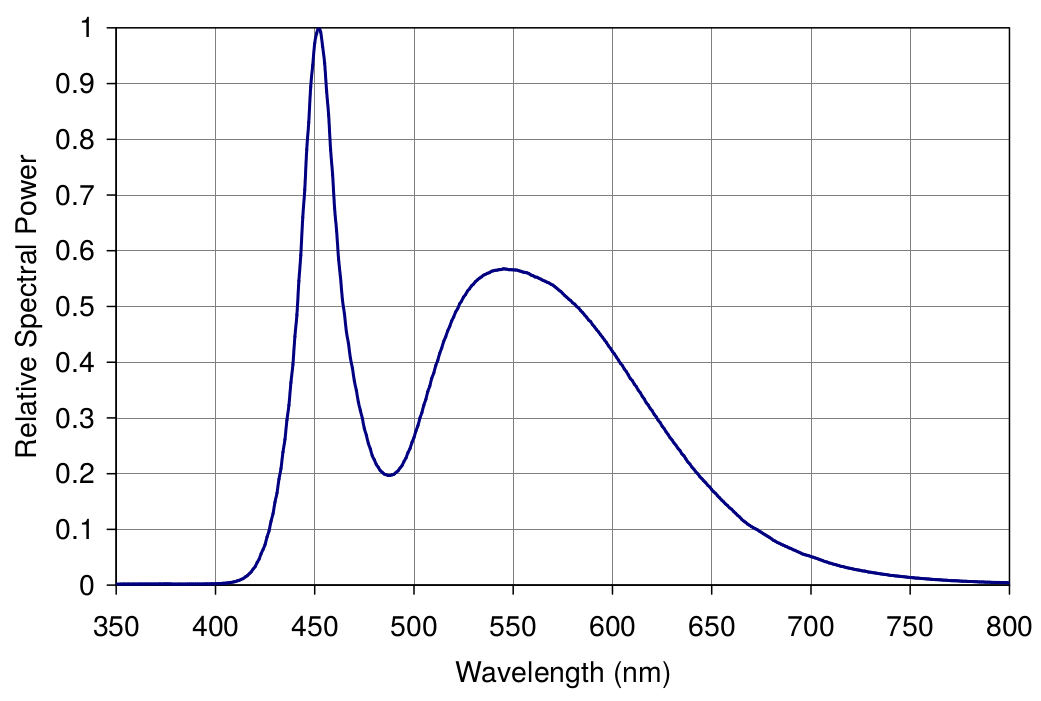
\includegraphics[width=0.8\linewidth]{./figs/chap2/ledspec}
	\caption[Typical relative spectral intensity of the LEDengine LED at an operating temperature of \SI{25}{\degreeCelsius}.]{Typical relative spectral intensity of the LEDengine LED at an operating temperature of \SI{25}{\degreeCelsius}, taken from the vendor's supplementary information~\cite[p. 10]{ledengin}.}
	\label{fig:ledspec}
\end{figure}
In order to allow for saturating illumination of the sample, the choice of light source is crucial and it was thus a main focus of this part of the project to identify such a source and to successfully connect it to the combination of Lakeshore cryogenic station and \McA{} Kelvin Probe. Successful \spv{} measurements are routinely carried out in the group using the Ambient Kelvin Probe Station and its xenon-lamp. The xenon-lamp is not only a source of light, but also a source of heat and thus unsuitable for the temperature-dependent measurement inside the \McA{}. Not only would the heat introduce uncertainties in temperature but temperature gradients introduced by it could also damage the cryostation, specifically the radiation shielding stage's sapphire window. Therefore, the choice fell upon a high intensity, natural-white light emitting diode (\led{}) manufactured by \led{} Engin, model LZP-00CW0R. The LEDEngin \led{} uses 25 \led{}-spots soldered onto and electrically connected by a printed circuit board (\pcb{}). Using thermo-paste, the \led{} is mounted onto a copper-core of a discarded computer fan. The fan is driven by a motor that uses a small 12V AC current source to achieve the necessary cooling of the delicate \led{}. As purchased, the \led{} has a relatively wide illumination cone of \ang{60}, due to an internal fish-eye lens that is situated right atop the \pcb{}. Therefore, the lamp was supplemented by a total internal reflection lens by LEDEngin that focuses \SI{90}{\percent} of the illumination into a \ang{10} wide cone. The initial \led{} of nominally \SI{4200}{\lumen} intensity was damaged, only 12 of 25 \led{}-spots were functioning and was later replaced by new \led{} of the same manufacturer with \SI{5400}{\lumen} intensity. The \led{} is driven by a variable DC source at a maximum voltage of \SI{18.2}{\volt} and maximum current of \SI{1.5}{\ampere}. Its relative spectral intensity is given in Figure \ref{fig:ledspec}.


\section{Measuring \cpd{} at Room Temperature}
\subsection{Sample Preparation}
A fresh surface of \hopg{} is prepared by gently rubbing adhesive tape onto a square piece of \hopg{} and tearing it off evenly. The piece is mounted onto a sample-holder using an electrically conductive clip and the \cpd{} is measured.\\
n-\sih{} (100) with different resitivities/doping-levels is prepared according to a slightly modified standard cleaning procedure: pieces of suitable size are cut with a diamond tip cutter, swiped off with ethyl-acetate and successively sonicated for three minutes each in ethyl-acetate, acetone, methanol and water. The pieces are microwave-treated in an \oxy{}-plasma at \SI{100}{\watt} with a flow of \SI{1}{\cubic\centi\metre\per\minute} \oxy{} and \SI{1.5}{\cubic\centi\metre\per\minute} Ar for 3 minutes. Subsequently, samples are rinsed with pure water (\SI{18}{\mega\ohm\centi\metre} at \SI{20}{\degreeCelsius}), immersed in \SI{2}{\percent} HF etching solution for 1 minute, rinsed with water and ashered again as before. The pieces are etched as before, back-contacts are created by applying InGa-eutectic to a scratched back surface. The piece is mounted onto a sample holder and the \cpd{} is measured for at least two minutes each on three different spots per piece. The time the sample is subjected to ambient after etch and before each measurement is recorded and used in a linear fit \lq{}$\Delta (\cpd{})/\Delta \, t$\rq{} to serve as an indication of the \cpd{} each spot on each piece would have had right after the etch, i.e. without the time needed for creating the back surface, mounting the sample and measuring other spots.
\subsection{Results \& Discussion}
The standard deviation of measured \cpd{} between spots of the same piece is comparable to that between pieces, so all obtained values were averaged. The values obtained across the three systems agree very well with each other and in the case of mid- and high-resistivity silicon also with theory, see Figure \ref{fig:nsih}. A three,  instead of only one, minute long HF etch did not influence the \cpd{} obtained for the low resistivity sample. A possible explanation for the deviation from theory might be found in the increased surface-reactivity of highly doped silicon: by the time the experiments are started, the silicon surface might already be oxidised. 
\begin{figure}
\centering
	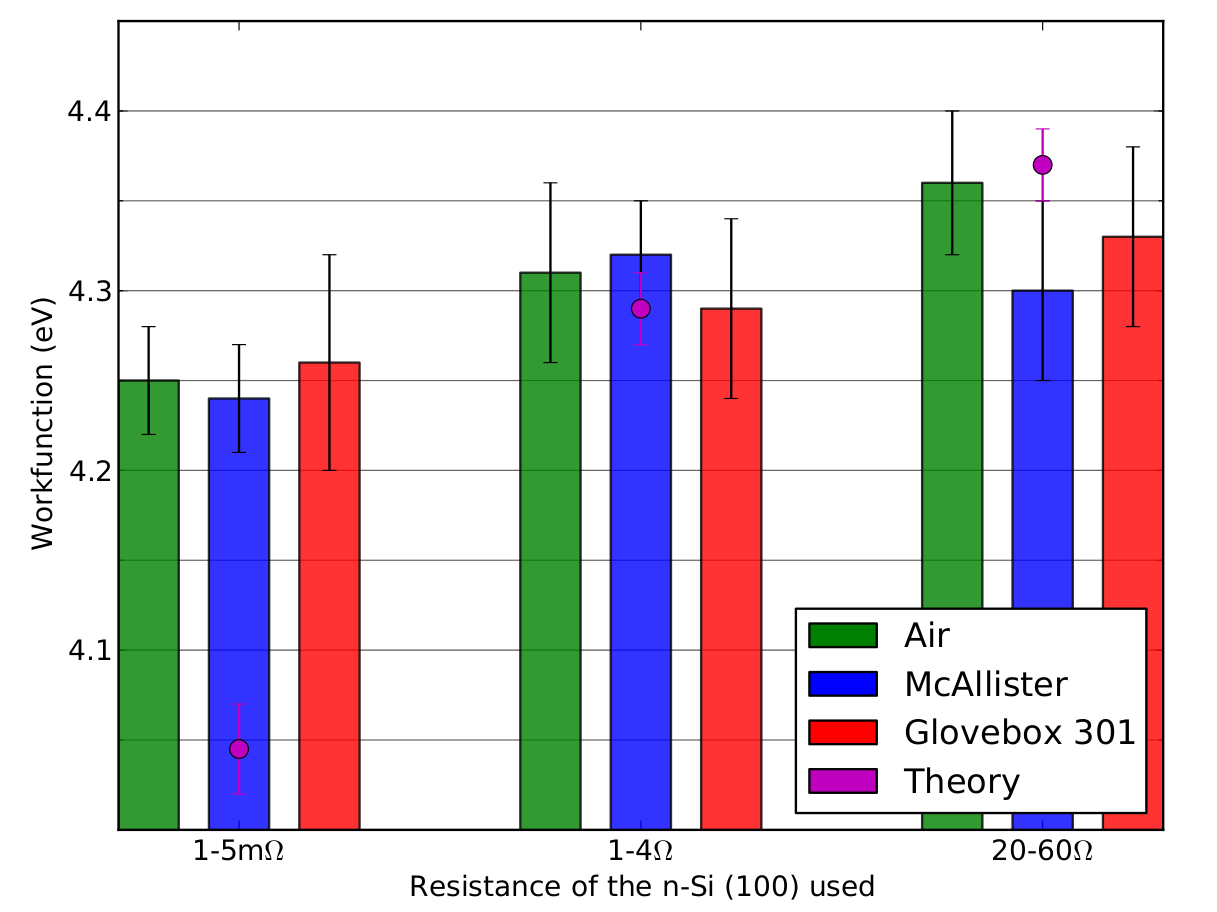
\includegraphics[width=0.8\textwidth]{./figs/chap2/Sih}
\caption{Summary of the calculated work functions for the n-\sih{} samples used. There is good agreement between the different systems and good agreement with theory, except for the case of low resistivity, highly doped silicon. Indicated errors include deviations in the samples \& the inaccuracy of calibration with \hopg{}.}
	\label{fig:nsih}
\end{figure}


\section{\cpd{} as Function of Pressure and Temperature}
\subsection{\cpd{} as a Function of Pressure}
Once it was established that results obtained from the three independent system under similar conditions using hydrogenated silicon as a reference sample, efforts were concentrated on temperature and pressure dependent measurements in the Lakeshore cryogenic system. Because of unavoidable contamination with oxygen from ambient, hydrogenated silicon was not used to that end. Instead, a freshly prepared reference of \hopg{} was placed on the ground of the radiation shielding stage without a sample-mount. An electrically conductive screw and clip were used to connect the top of the \hopg{} sample to the electrical ground of the Lakeshore. Two sets of experiments were carried out to independently determine the influence of pressure and temperature on the measured \cpd{}. In the first set, the measurements was commenced under ambient condition and allowed to continue for some time. The probe head was then retracted to avoid crashing it onto the sample and the weak pump was turned on. The probe head was then brought into proximity of the sample to continue the measurement and the measurement was allowed to continue for some time. The probe head was retracted again and the turbo pump was switched on. Again, the probe head was lowered to continue with the measurement and the measurement was allowed to continue for some time. For results of this experiment, see Figure \ref{fig:hopg-p}.
\begin{figure}
\begin{subfigure}{0.5\textwidth}
\centering
	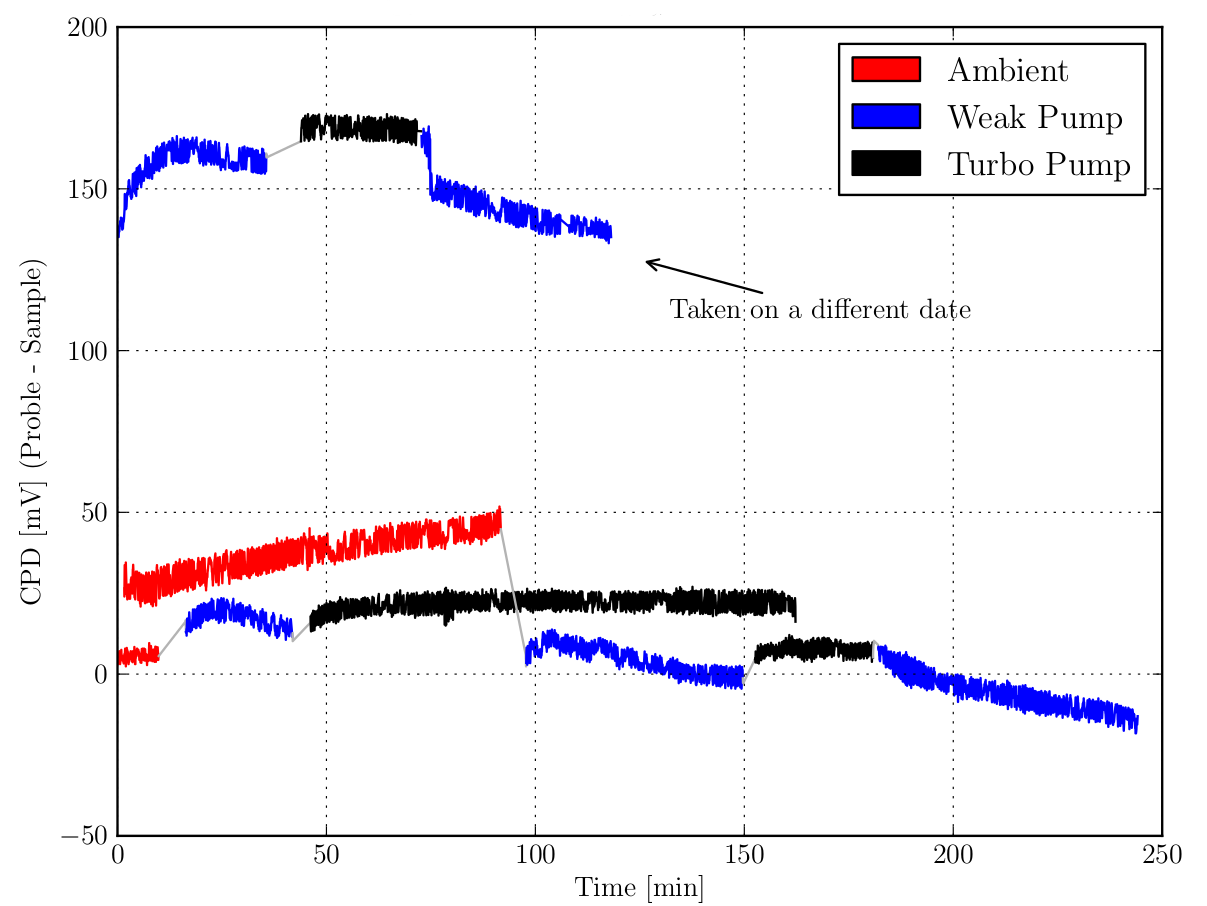
\includegraphics[width=0.95\linewidth]{./figs/chap2/HOPGMcA}
	\caption{}
	\label{fig:hopg-p1}
\end{subfigure}
\begin{subfigure}{0.5\textwidth}
\centering
	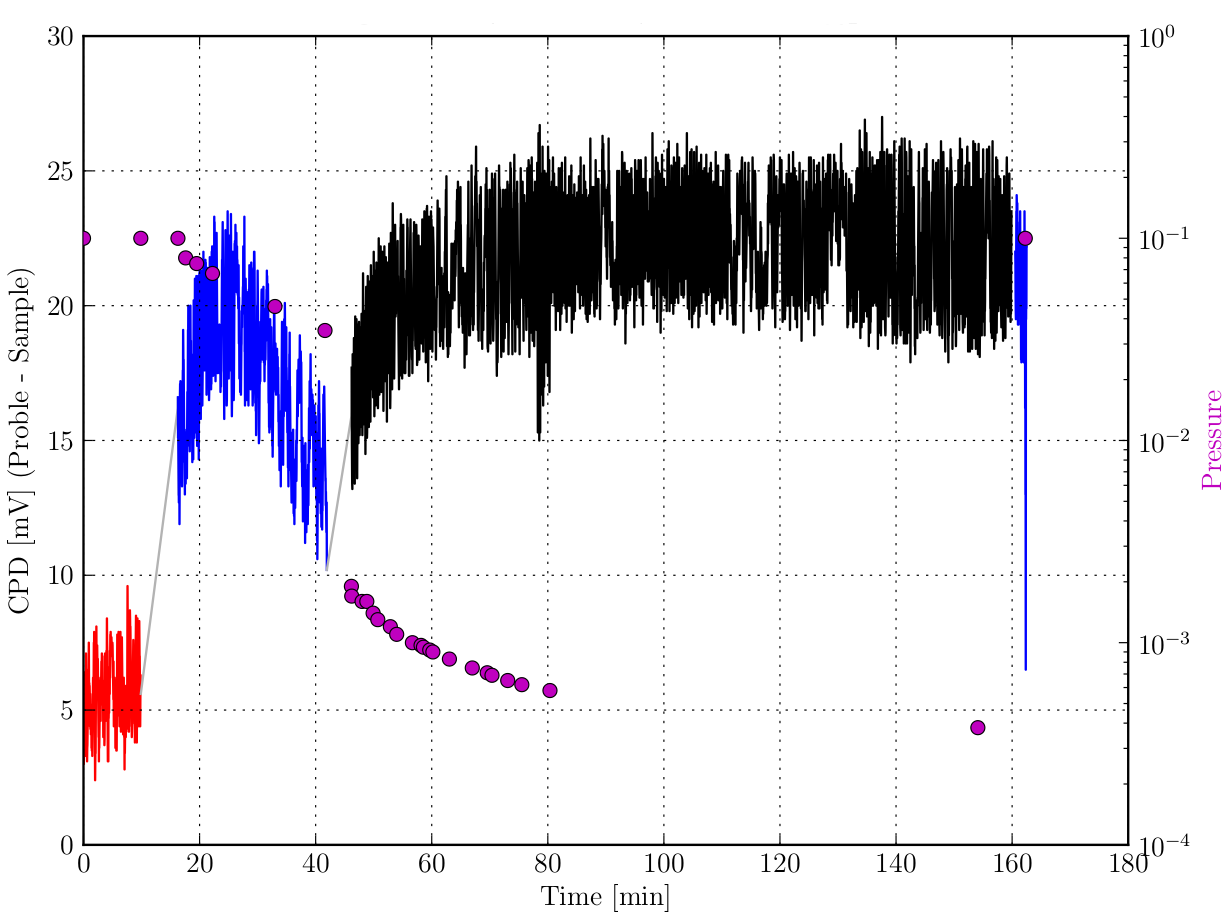
\includegraphics[width=0.95\linewidth]{./figs/chap2/HOPGMcAPres}
	\caption{}
	\label{fig:hopg-p2}
\end{subfigure}
\caption{Raw data obtained from a measurement of the \cpd{} during pressure reduction in the \McA cryogenic system. Figure \ref{fig:hopg-p1} shows results obtained from independent measurements of a piece of \hopg{} carried out on different days. It is indicated which pump was active to reduce the pressure inside the sample chamber. Figure \ref{fig:hopg-p2} gives more detail about one of these measurements and actual measurements of the pressure at different stages during evacuation.}
\label{fig:hopg-p}
\end{figure}
This experiment revealed several features. Firstly, the \cpd{} of \hopg{} rises as a function of time under ambient condition. This is readily explained by oxygenation and/or other sources of contamination from ambient, such as water for example. Once the weak pump is turned on, there is a discontinuity in \cpd{}. This discontinuity is not systematic in its direction, it may change the \cpd{} either 'up' or 'down' and can therefore best be explained by a displacement of the probe head over the sample. The sudden reduction in pressure exerts a force on the probe arm and may cause it to move slightly. The size of the discontinuity is within the size of variation of \cpd{} observed when different spots of the same reference are measured. The \cpd{} now reduces as a function of time and this may be explained by gradual decontamination of the sample: as the pressure reduces, previously adsorbed contaminants may leave the surface. A second viable explanation may be a gradual change in acoustic vibration characteristics as a result of the reduction in pressure. To distinguish between the two, an experiment was performed in which the sample chamber was flushed with clean, inert Argon after having been subjected \uhv{} conditions for about 20 minutes. It is assumed that complete desorption of possible contaminants is achieved by this treatment and that the high purity argon does not introduce fresh contaminates. The pressure was then again reduced using the weak pump and the \cpd{} again reduces as a function of time. We therefore conclude that the observed reduction in \cpd{} is indeed caused by gradual changes in pressure rather than desorption of contaminants. It is thus advisable to carry out \cpd{} experiments under conditions of stable pressure, especially given the fact that the probe head is specifically designed by \McA{} to carry out ultra-high vacuum \cpd{} measurements. 
\subsection{\cpd{} as a Function of Temperature}
To determine the possible influence of temperature on the quality and reliability of the measurement, a \SI{30}{\nano\metre} thick layer of AlO$_3$ was grown on an n-type silicon wafer by plasma-enhanced atomic layer deposition (\peald{})~\cite{ann_inversion2}. Alumina was chosen as a surface of interest because of its natural affinity for water. If contamination by water and subsequent freezing of the surface is an inherent problem of low temperature \cpd{} measurements, then a strongly hydrophilic surface should exhibit these problems. Pieces of suitable size were cut from the wafer and swiped off with ethyl-acetate and sonicated for three minutes in iso-propanol, blow-dried under \nitro{} and subsequently microwave-treated in an \oxy{}-plasma at \SI{100}{\watt} with a flow of \SI{1}{\cubic\centi\metre\per\minute} \oxy{} and \SI{1.5}{\cubic\centi\metre\per\minute} Ar for 3 minutes, ensuring a clean alumina surface. The back-side was scratched and InGa-eutectic was applied to create a back-contact. The work-function of this surface was measured in the ambient probe station and found to be \SI{4.42+-0.03}{\electronvolt}. To ensure an ohmic back-contact, the sample stage of the Lakeshore was lightly scratched and a small quantity of InGa-eutectic was applied to the stage. The piece was then placed on the sample stage and slight pressure was applied. The stage was introduced into the Lakeshore cryogenic system and the pressure was reduced. Using liquid nitrogen and the heaters, the temperature was reduced to \SI{250}{\kelvin} and allowed to stabilise. Under these conditions, the work-function of the alumina surface was found to be \SI{4.44+-0.04}{\electronvolt}~\footnote{A suitable piece of \hopg{} was also present in the sample chamber to allow for calibration of the work-function of the probe head}. It has to be pointed out that the sample surface is not the coldest point inside the Lakeshore's inner chamber. Because of the way liquid nitrogen is introduced into the system, the radiation chamber's ground surface is the coldest. Therefore, it can be assumed that any ice would form there rather than on the sample, corroborating the result presented above.
\subsection{Conclusion}
\cpd{} measurements using the Lakeshore are feasible when the pressure is constant. They may be carried out under ambient pressure with an inert argon atmosphere or under ultra-high vacuum conditions. A changing pressure is not conducive for reliable measurements of the contact potential difference but under conditions of stable pressure, \cpd{} values obtained from the Lakeshore agree with values obtained from the other probe stations. Lowering the temperature below the freezing point of water does not pose an inherent restriction on the feasibility of \cpd{} measurements in the Lakeshore system. The observed \cpd{} was in agreement with experiments carried out at room temperature. In agreement with the literature~\cite{tempdepmet,tempdepmet2,tempdepmet3,tempdepmet4,tempdepmet5} possible fluctuations of the work function of the probe head are small compared to other sources of experimental uncertainty and the \wf{} can indeed be taken as a constant.


\section{Measuring the \spv{} at Room Temperature}
A necessary condition for the successful determination of the \spv{} of a sample is saturation with light. In practice, this means that the light-intensity during a measurement of the \spv{} is gradually increased up to the point where further increase in intensity does not lead to further increase of the measured surface photovoltage. Detailed interpretation of the measured signal is often problematic and requires intimate knowledge of the sample and even theoretical discussions of the \spv{} tend to be very involved. However, from the point of view of establishing whether a new experimental set-up is suitable for more advanced \spv{}-measurements, a successful, saturated measurement of the \spv{} of a relatively simple test-sample is a necessary precondition. To that end, \spv{} measurements of an alumina surface were chosen as a test case. Alumina was chosen for its stability, relative simplicity and because of its relatively large \spv{} signal. The sample is the same as used for the determination of the temperature dependence of the \cpd{}: \SI{30}{\nano\metre} AlO$_3$ was grown on an n-type silicon wafer by \peald{}. The preparation and cleaning protocol of the sample is the same as above: rinsing; sonication; oxidation and creation of an ohmic back-contact using InGa-eutectic. The sample's \spv{} was determined in the ambient probe station as is~\footnote{i.e. ambient probe station and xenon light source} and was found to be \SI{530+-20}{\milli\volt}. To check if the \led{} is a suitable source, it was installed in the ambient probe station and an \spv{} measurement was carried out. To facilitate the comparison between the systems, the ambient probe station's light focusing lens was removed as no such lens could readily be installed with the Lakeshore. Since the \led{} has a variable electrical source, it was possible to increase the current through the \led{} from \SIrange{1}{1.6}{\ampere} in steps of \SI{0.1}{\ampere}. In a set of preliminary experiments not reported here, it was established that the illumination intensity of the \led{} as determined from a standard silicon test-cell does indeed increase smoothly over the appropriate current range. The sample was introduced into the Lakeshore's inner chamber and the \led{} was placed on top of the vacuum chamber's outer window. The current through the \led{} was increased in the same steps as for the measurement in ambient and the results of the experiment are summarised in Figure \ref{fig:Iseries}.
\begin{figure}
\centering
	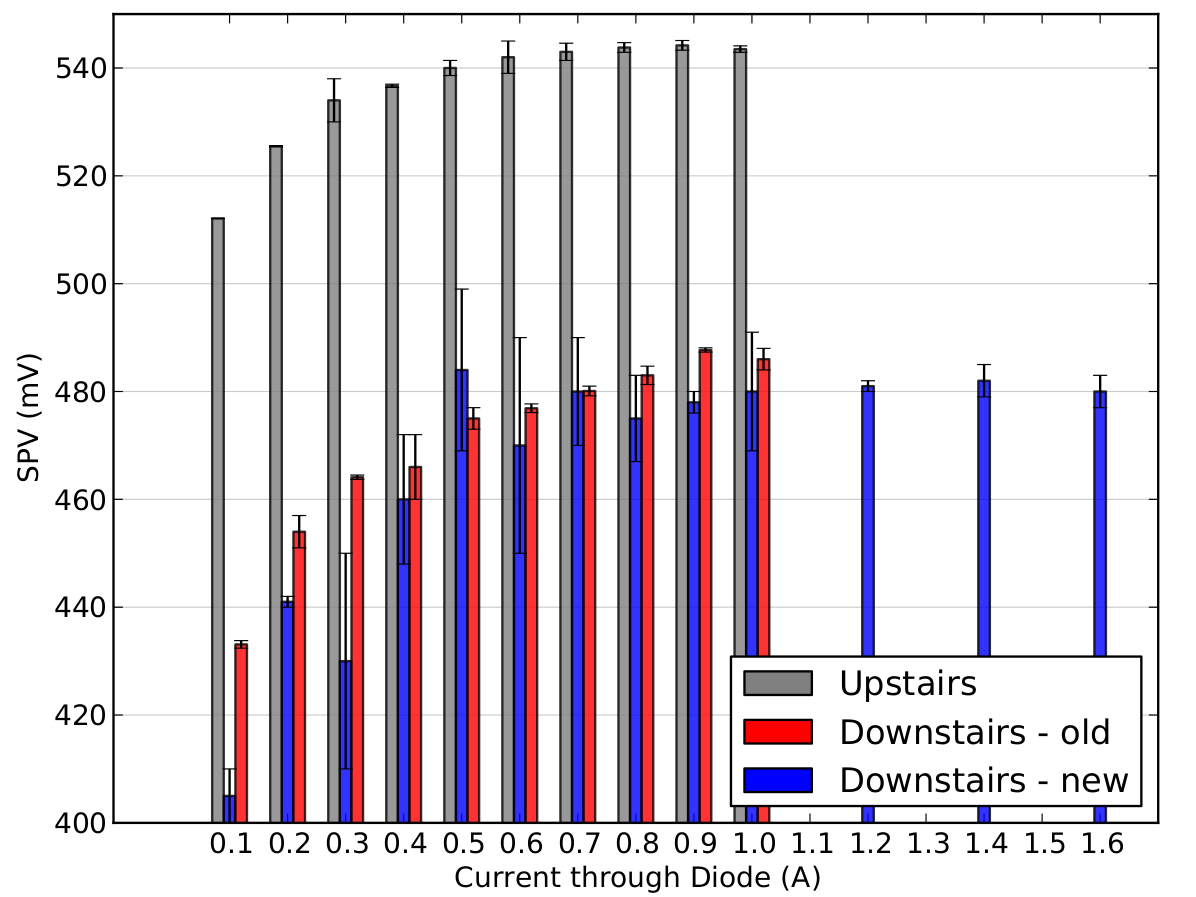
\includegraphics[width=0.8\linewidth]{./figs/chap2/currentseries}
	\caption{Comparison of the measured \spv{} as a function of illumination level as evidenced by the current through the \led{}. \enhyphen{Upstairs} refers to the combination of \led{} and the ambient probe station, while \enhyphen{Downstairs} refers to measurements with the \led{}, the \McA{} cryostation and the custom Lakeshore \kp{} probe head. \enhyphen{Old} signifies the weaker, damaged \led{} of nominally \SI{4200}{\lumen} intensity, while \enhyphen{new} refers to the fully functional \led{} of \SI{5400}{\lumen} intensity. Note that the measurement saturates independent of illumination intensity (\enhyphen{old} vs. \enhyphen{new}) at a lower measured \spv{} than the comparison with the ambient probe station.}
	\label{fig:Iseries}
\end{figure}
In that Figure \enhyphen{Upstairs} refers to the measurement in the ambient probe station, 'Downstairs' refers to the measurement with the \McA{} probe head, \enhyphen{old} refers to the initial \led{} with only 12 of 25 spots working and \enhyphen{new} refers to the newly purchased \led{} in which all diodes are working and which achieves a maximum illumination of \SI{5200}{\lumen}. It has to be pointed out that the new \led{} could be driven further than up to a maximum of \SI{1.0}{\ampere} to reach its full illumination intensity at a maximum current of \SI{1.6}{\ampere}, so the experiment was extended to make use of the maximum achievable intensity. As can be seen, saturation of the \spv{} is readily achieved with the \led{} in ambient at a current of \SI{0.6}{\ampere} and the measured value of \SI{540+-10}{\milli\volt} is in good agreement with the value expected from the measurement of the \spv{} with a xenon light source. It is furthermore apparent that the measurement achieves saturation. At a current of about \SI{0.8}{\ampere}, a further increase in current does not result in a corresponding significant increase in measured surface photovoltage. However, there is a significant discrepancy of \SI{60}{\milli\volt}~\footnote{about \SI{10}{\percent} of the maximum signal} in measured \spv{} between the two systems which cannot readily be explained. A similar experiment using neutral density filters to control the light intensity was carried out, but no meaningful conclusions could be drawn from the results, so it is not presented here. In a following step, the \spv{} of the alumina sample was measured with the Lakeshore not completely assembled. The vacuum chamber's lid as well as the radiations shielding chamber's lid were removed and the \led{} was held by hand as close to the probe head as possible without interfering with the measurement~\footnote{a constant stream of argon was employed to avoid undue contamination of the inner chamber from ambient.}. This configuration obviously does not represent a working condition for the Lakeshore, nor is it readily reproducible because of its vague parameters, but an \spv{} of $\sim$ \SI{480}{\milli\volt} could be achieved in this way. At this point, the nature of the \SI{60}{\milli\volt} discrepancy remains unknown. It might be due to the increased distance between the source and the sample or it might be due to partial absorption by the Lakeshore's windows, especially the \ir{}-shielding sapphire glass but the results obtained here remain hard to interpret properly. Saturation is achieved, but not at the right level. Simply using a stronger source will therefore most likely not alleviate the problem. It may be tried to replace the windows by lenses which better focus the light beam onto the sample but is is questionable if such a scheme is practically feasible or indeed even helpful. Practically, such window-lenses would have to be able to withstand \uhv{} conditions and saturation was achieved in ambient even without a lens, where the distance between sample and source is comparable to the corresponding distance in the cryogenic system. Since no explanations of the source of the discrepancy between the systems are forthcoming, a systematic experimental uncertainty of underestimating the \spv{} by about \SI{10}{\percent} has to be assumed when using the Lakeshore in conjunction with the \led{}.


\section{Temperature dependent Measurement of the \spv{}}
Since it was established that temperature dependent \cpd{} measurements could reliably be carried out and that, albeit with a systematic uncertainty, \spv{} measurements could also be carried out with the Lakeshore cryogenic system, the final step was to attempt a combined experiment and carry out a temperature dependent measurement of the surface photovoltage. To this end, a suitable sample needed to be identified. This sample should have a sufficiently large photo-response and should undergo some phase transition at a well defined, critical temperature. Three different systems were investigated: biological samples consisting of a plant's photo-system immobilized on a gold surface; a lead-iodide-chloride perovskite on titanium-dioxide and finally a thin layer of vanadium oxide.\\
The biological samples exhibited changes in \cpd{} on the order of \SI{20}{\milli\volt}. These changes occurred at a well defined temperature, from \SIrange{250}{260}{\kelvin}. While interesting, these changes but were too small to serve as a reliable system for a proof of principle: \SI{20}{\milli\volt} is within the experimental uncertainty of both the \cpd{} and the \spv{} measurements. The biological samples were therefore quickly abandoned.\\
For the perovskites, it was attempted to compare their reaction when exposed to different parts of the optical spectrum, namely to compare their dark \cpd{} to the \cpd{} when exposed to full spectrum illumination and when exclusively exposed to infra-red illumination. The perovskite sample was introduced to the inner chamber of the Lakeshore and electrically contacted with the help of a conductive clip and screw. To allow for electrical connection via the back contact, the perovskite was removed from the point where the clip contacted the sample. The cryogenic system was evacuated and seven temperatures where chosen at which to measure the \cpd{}: \SIlist{130;170;210;230;250;270;280}{\kelvin}. At each of these temperatures, the dark \cpd{} was measured. A filter which would only allow \ir{} radiation to pass was placed in front of the source, the sample was briefly illuminated and the \ir{} \cpd{} was measured. The \cpd{} of the system was allowed to decay back to its original dark value and the filter was removed. The system was then briefly illuminated by full spectrum at high intensity and the light \cpd{} was measured. The \cpd{} of the system was allowed to decay back to its original dark-value and the system was then cooled down to the next temperature step. In the course of this measurement, repositioning the probe head to new positions over the sample was necessary because although care was taken, crashing the probe head onto the sample could not be avoided. The whole experiment was carried out under low pressure conditions, but for the lowest five temperature points, the pressure was about a factor ten lower than for the measurements taken at \SIlist{270;280}{\kelvin}. To carry out the experiment, the set up of the \McA{} had to be modified twofold. Measurements had to be carried out without the inner chamber's sapphire glass window as this would exclude any infra-red radiation from reaching the samples in the first place. Secondly, the xenon lamp had to be used as a source of illumination to give access to the infra-red part of the spectrum. These modifications introduced experimental difficulties for several reasons. As already pointed out, the xenon lamp is a source of heat and therefore, an unknown experimental uncertainty in the temperature was introduced. The experiment had to be carried out very quickly to avoid damage to the system and to minimize said uncertainty in temperature. In effect, only a brief flash of illumination could be allowed to reach the sample. Furthermore, the xenon lamp and its high power electrical source had to be set up in close proximity to the Lakeshore cryogenic system and electrical noise due to the relatively high currents and voltages involved in this experiment were introduced. To add to these problems, the sample was neither fresh nor necessarily stable and perovskites are inherently complicated systems. Accordingly, the results did not show a clear variation with temperature and could not be reproduced on consecutive days. Therefore, it was decided that this experiment could not serve for the purpose of showing a reliable \spv{}(T) measurement.\\

\subsection{Vanadium Oxide}
\label{sec:vox}
\subsubsection{Description of Samples and preliminary Research carried out at the Cahen Group}
Vanadium-dioxide (\vadiox{}) is a system well known for undergoing a metal to insulator transition (\mit{}) close to room temperature. At the heart of this transition lies a reconfiguration of the of the crystal lattice, where \vadiox{} transitions from its high-temperature tetragonal (rutile) phase to a low temperature monoclinic phase. In the tetragonal phase, the Fermi level of the material is well within the conduction band and hence, the material behaves like a metal. In the monoclinic phase, an energy gap has developed and the material now behaves like an insulator~\cite{nakano_gapopen}. Of course, the only difference between an insulator and a semiconductor is the size of their energy gaps and if the transition occurs gradually, one might also speak of a metal-semiconductor-insulator transition instead of an \mit{}. This transitions has extensively been studied, using many different methods such as direct photoemission \& x-ray absorption spectroscopy~\cite{koethe_expstud}, Raman spectroscopy~\cite{radue_raman}, ultra-fast pump-probe spectroscopy~\cite{jensen_expgap} etc. However, because of their relative simplicity, studies of the resistivity of the material stick out~\cite{shibuya_physlet}. In these, changes of resistivity over several orders of magnitude are not uncommon. Finally, the \mit{} in \vadiox{} was also investigated using Scanning Kelvin Probe Microscopy, where $\sim$ \SI{200}{\nano\metre} thin stripes of the material were grown adjacent to a strip of gold. These strips were continuously scanned over a temperature range including the phase transition temperature ($T_{MI}$) of \vadiox{}. Gold provided a stable reference work function and thus, the work function of \vadiox{} could be measured in absolute terms. It was found that vanadium-dioxide has a work function of $\sim$ \SI{5.15}{\electronvolt} in its metallic phase and that the work function gradually decreased by $\sim$ \SI{0.15}{\electronvolt} over a range of \SI{60}{\kelvin}~\cite{ko_kp}. In other studies~\cite{shibuya_physrev}, it was found that \mit{} could be tuned by tungsten-doping of a thin film of \vadiox{} grown on a supporting matrix of \tiox{} and preliminary research into similar samples has already been carried out in the Cahen group.\\
The samples were either pure or \SI{2}{\percent} tungsten-doped vanadium-dioxide of thickness ranging from \SIrange{10}{80}{\nano\metre} grown on either \tiox{} or on niobium-doped titanium-dioxide (Nb:\tiox{}) and were kindly provided by M. Nakano of RKIEN. A change in resistivity of several orders of magnitude upon \mit{} could be shown for these samples. When used for this project, however, the collection of vanadium-dioxide samples had already been in storage inside a desiccator for more than a year. Many samples were damaged and proper storage throughout the year could not be guaranteed. Therefore, the choice of sample for this project was limited to pieces which, upon optical inspection, were closest to their initial appearance and were still large enough to allow proper positioning of the probe head over a sufficiently homogeneous surface. Therefore, a sample of \SI{50}{\nano\metre} \SI{2}{\percent} \wvadiox{} on pure \tiox{} was chosen. It had been investigated by Nir Kedem using the van der Pauw method with a temperature resolution $<$\SI{5}{\kelvin}. It showed an approximately two orders of magnitude change in resistivity with a relatively gradual profile, occurring over the temperature range from \SIrange{220}{270}{\kelvin}. The resistivity also exhibited hysteresis, with up to half an order of magnitude difference in resistivity between cooling down and heating up.
\subsubsection{Experimental Procedure, Results and Discussion}
Initially, the work function of the vanadium-dioxide sample was determined with the ambient probe station. The sample was sonicated for three minutes each in acetone, ethanol and THF and was then blow-dried under \nitro{}. To calibrate the probe head, a fresh surface of \hopg{} was prepared and the \cpd{} was measured. The work function of the probe head was found to be \SI{5.085+-0.015}{\electronvolt}. The work function of the clean \wvadiox{} sample was determined to be \SI{5.17+-0.02}{\electronvolt}, in remarkable agreement with the value obtained by Ko \emph{et~al.}~\cite{ko_kp}.\\
Before each measurement, the sample was subjected to the same cleaning procedure outlined above. The sample was then blow-dried under \nitro{} and placed directly on the ground of the inner chamber of the Lakeshore. Electrical contact was made from the top using a conductive screw and clip. The Lakeshore was then evacuated and the experiment commenced once a stable vacuum condition was obtained.\\
In the first experiment, the Lakeshore was cooled down to the lowest temperature achievable by liquid nitrogen cooling: \SI{97}{\kelvin} for this cryogenic system. During this cool-down, the \cpd{} was quickly measured at three points where the temperature remained relatively stable for a sufficient time. Once the lowest possible temperature was reached, the flow of nitrogen was stopped, the heater was set to \SI{300}{\kelvin} and the \cpd{} was measured continuously. This protocol allows for a quick measurement of the \cpd{}(T)-response of the system to identify the temperature range of interest, but uncertainties in temperature are introduced because of the temperature gradient present in the inner chamber and because of having to note down the temperature manually. The experiment had to be aborted. The data obtained during this initial experiment are shown in Figure \ref{fig:vox1}.\\
\begin{figure}
\centering
	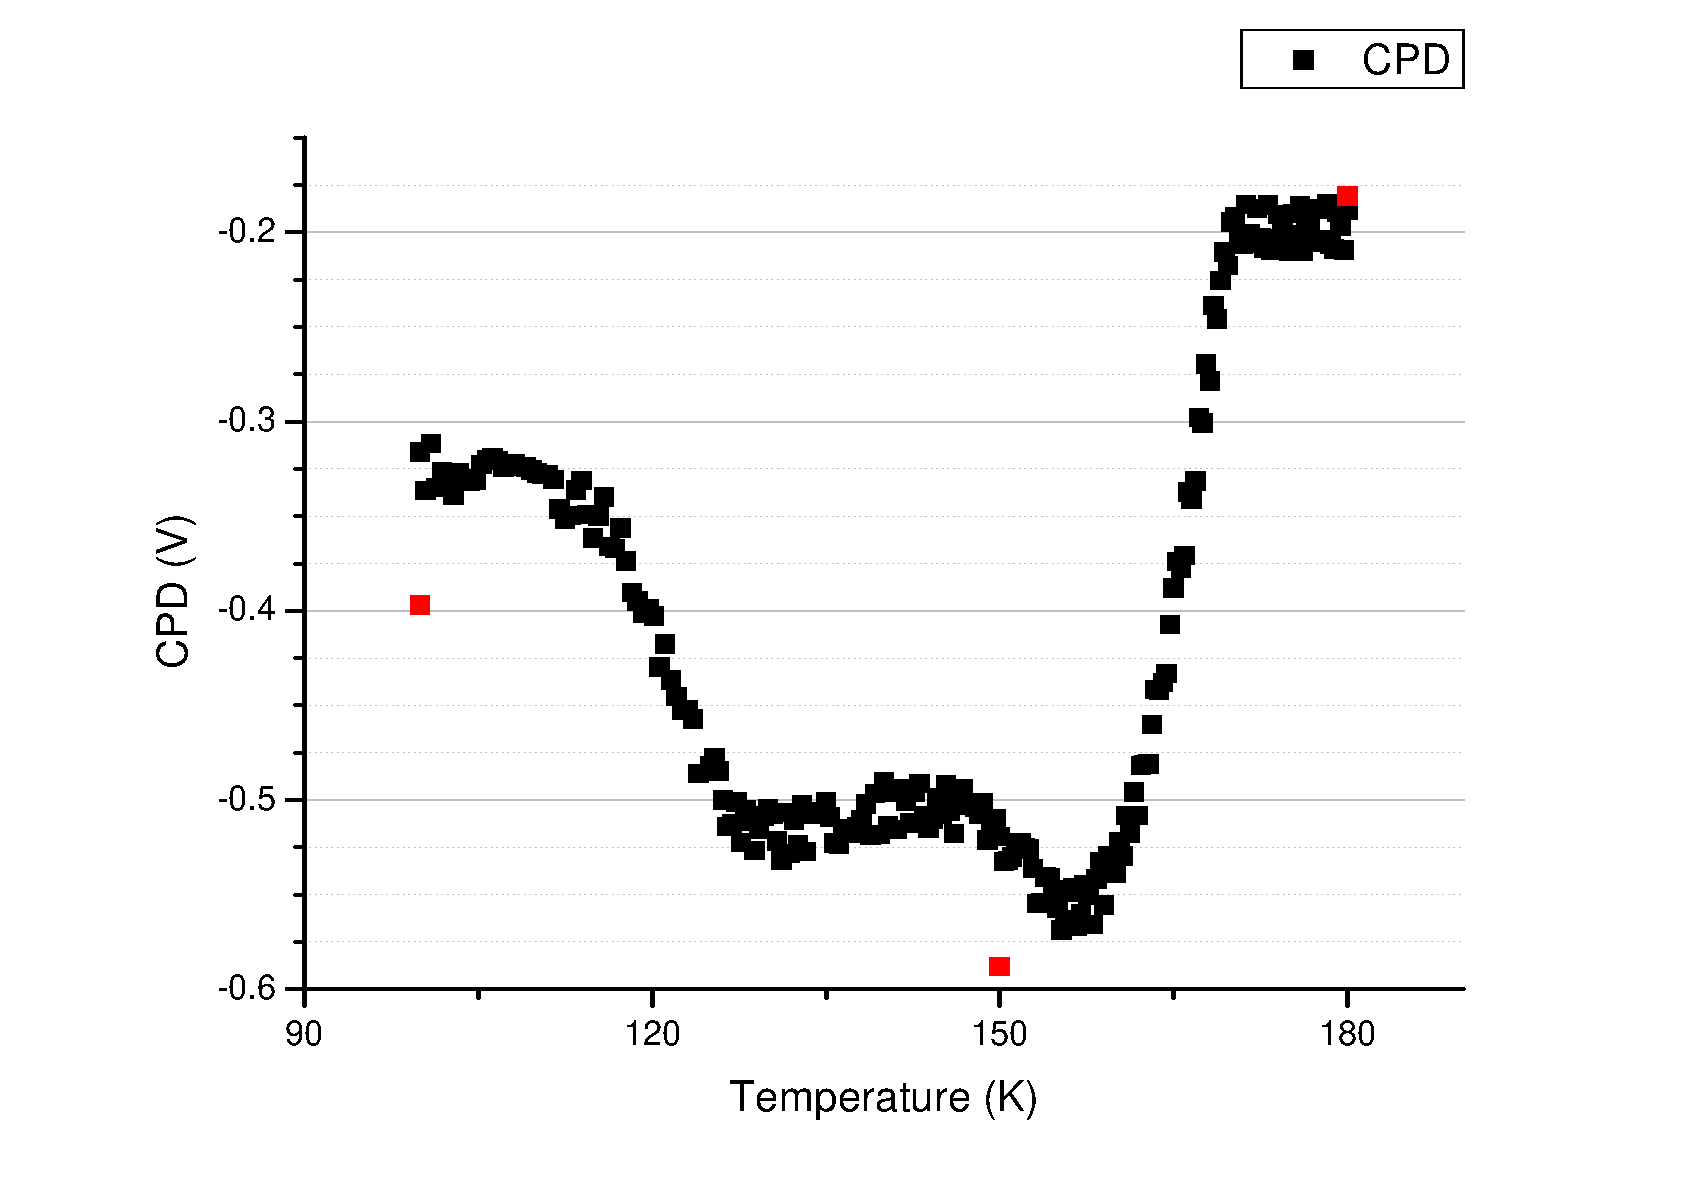
\includegraphics[width=0.8\linewidth]{./figs/chap2/vox1}
	\caption{Raw data of the contact potential difference of the \wvadiox{} sample obtained during a temperature-sweep. Data points in red were obtained while cooling down, data points in black were recorded while warming up.}
	\label{fig:vox1}
\end{figure}
For the next experiment, the temperature range was extended and more care was taken to more accurately determine the temperature. The system was cooled down to \SI{100}{\kelvin} and gradually increased. The \cpd{} was measured at 11 well defined temperatures. For each of these temperatures, the flow of liquid nitrogen and the heater setting were carefully adjusted until all three of the cryogenic system's temperature read-outs were within a range of \SI{5}{\kelvin} of each other. Holding the temperature constant, the \cpd{} was then recorded once every second for a period of 100 seconds and these data were averaged. The temperature was increased to the next set-point and the procedure was repeated. The observations of this experiment are plotted in Figure \ref{fig:vox2}. The uncertainty in \cpd{} was taken to be twice the standard deviation of \cpd{} values obtained during the 100 second period. Uncertainty in temperature is not shown but assumed to be less than \SI{5}{\kelvin}.\\
\begin{figure}
\centering
	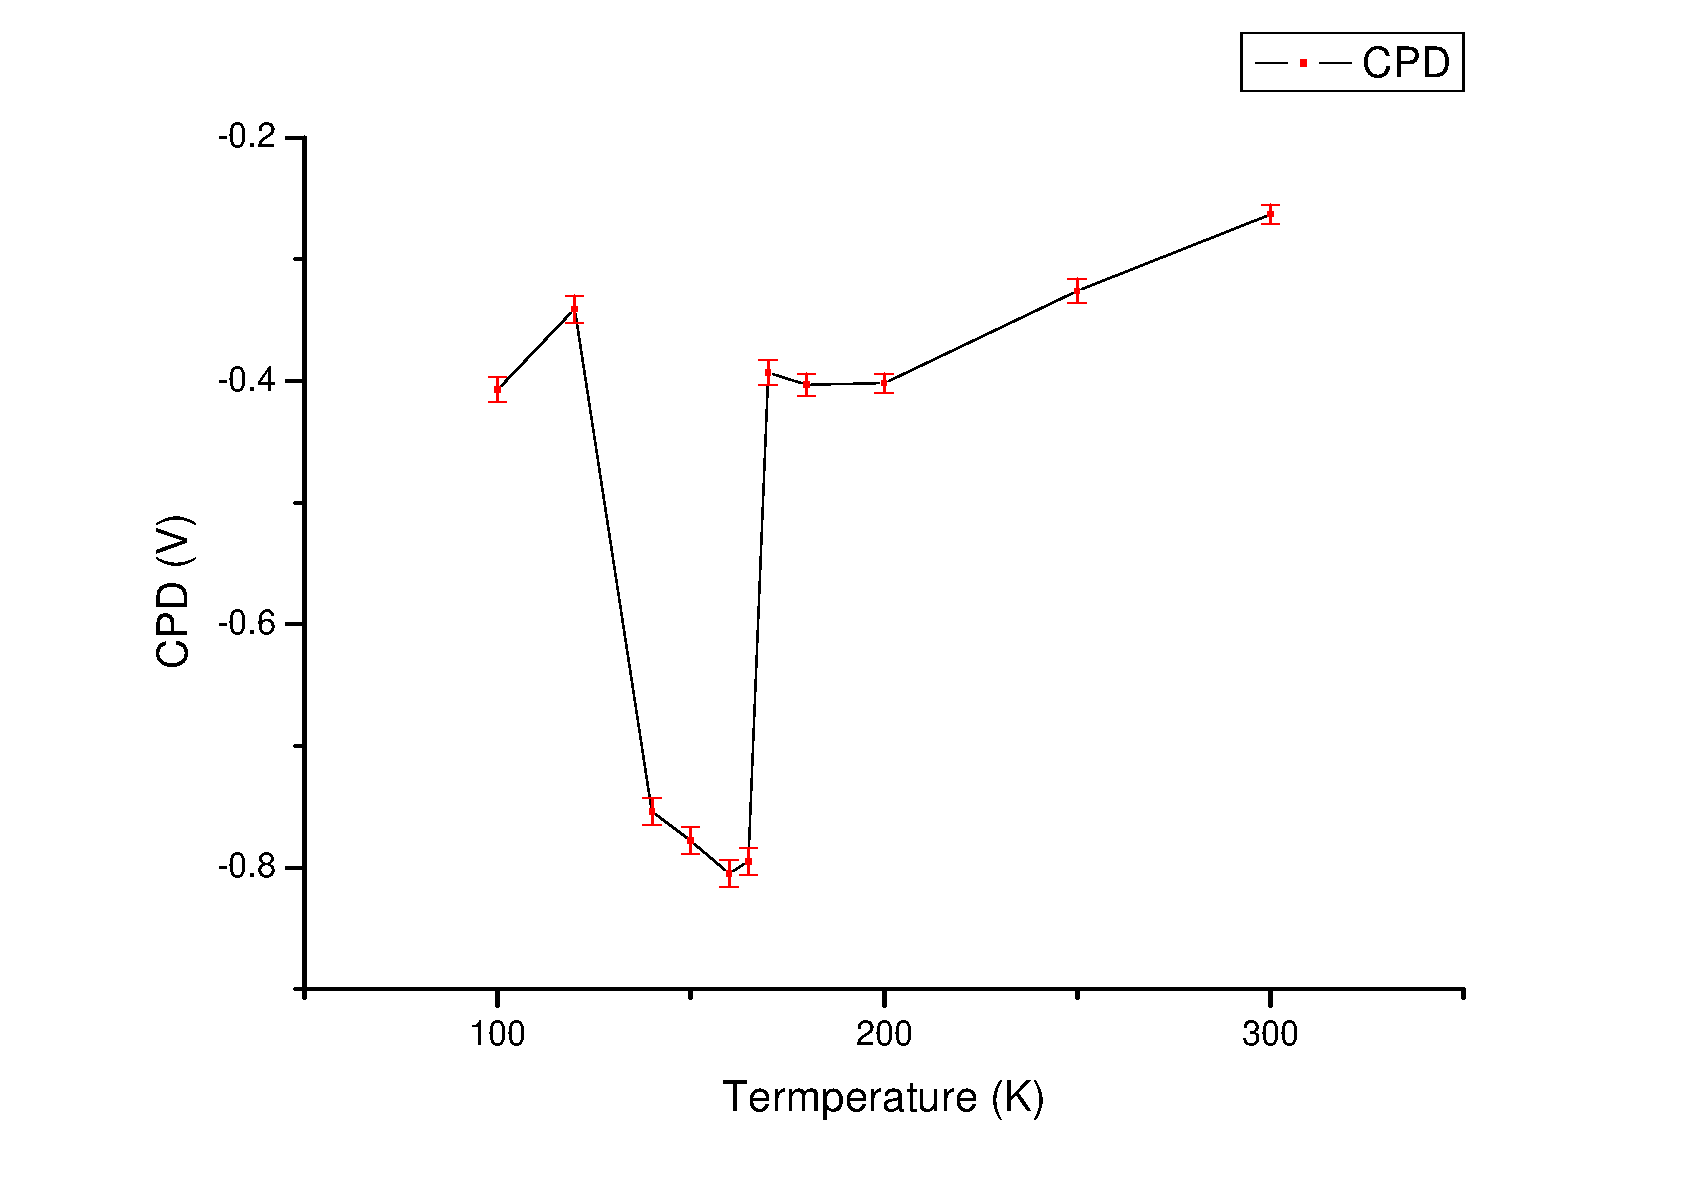
\includegraphics[width=0.8\linewidth]{./figs/chap2/vox2}
	\caption{The contact potential difference of the \wvadiox{} sample as a function of temperature. Experimental uncertainties are explained in the text.}
	\label{fig:vox2}
\end{figure}
In the last experiment, both dark and light \cpd{} were measured for the same sample for a range of temperatures between 180 and \SI{300}{\kelvin} in intervals of \SI{20}{\kelvin}. \cpd{} was only measured once the temperature gradient inside the Lakeshore was less than \SI{5}{\kelvin}. For each temperature, dark \cpd{} was measured once every second over a period of 100 seconds and these data were averaged. Illumination for light \cpd{} was achieved by the \led{} at maximum intensity and to avoid possibly heating the sample, light \cpd{} was measured for 15 seconds. \hopg{} as a reference for the work function was not used in this experiment. Instead, the work function of the sample at \SI{300}{\kelvin} in vacuum was assumed to be the same as that obtained from the same sample at room temperature in ambient and the work function of the probe could therefore be calculated to be \SI{4.41}{\electronvolt}. The results of this final experiment are shown in Figure \ref{fig:vox3}. The experimental uncertainty in work function includes twice the standard deviation of dark \cpd{} obtained during the 100 second interval plus an added uncertainty from the calculation of the work function of the probe head. The experimental uncertainty in \spv{} includes uncertainty from dark \cpd{} as well as that for light \cpd{}. Uncertainty in temperature is, again, not shown, but assumed less than \SI{5}{\kelvin}.\\
Probably the most remarkable feature of these measurements is the sudden drop in \cpd{} (sudden rise in \wf{}) at $\sim$ \SI{120}{\kelvin} and the consequent sudden rise in \cpd{} around $\sim$ \SI{170}{\kelvin} seen in both Figure \ref{fig:vox1} and Figure \ref{fig:vox2}. Since these features were observed during cool down as well as during heating up in the first and were again observed in the second, independent measurement, they are most likely not an artefact of the measurement, nor should they be ascribed to simple experimental failure. They represent a change in work function of $\sim$ \SIrange{200}{400}{\milli\electronvolt} which is remarkably large. Such changes can most likely not be explained by changes in shielding of accumulated surface-charges or repositioning of the Fermi level. A (reversible) surface-reconstruction or even a (reversible) change of chemical composition might be able to explain the data, but without further measurements, we cannot be sure. To the best of my knowledge, neither a structural reconstruction nor a change in \wf{} at the temperatures is question has yet been reported in the literature for \wvadiox{}. In conjunction with the measurements carried out by Nir Kedem, the experiments reported in the literature and those summarised in Figure \ref{fig:vox3}, it has to be assumed that the changes in \wf{} seen at around \SIlist{120;170}{\kelvin} are not explained by the known \mit{} of vanadium-dioxide. The difference in \cpd{} between heating up and cooling down seen in Figure \ref{fig:vox1} might be taken as evidence for hysteresis at lower temperatures than previously observed, but the data is sparse, so no conclusive explanation can be drawn from them. Figure \ref{fig:vox2} on the whole corroborates what was observed in the initial, relatively inaccurate experiment even though the size of the observed effect is greater. Nothing more about the origin of this effect can be concluded from these measurements alone.\\
\begin{figure}
\centering
	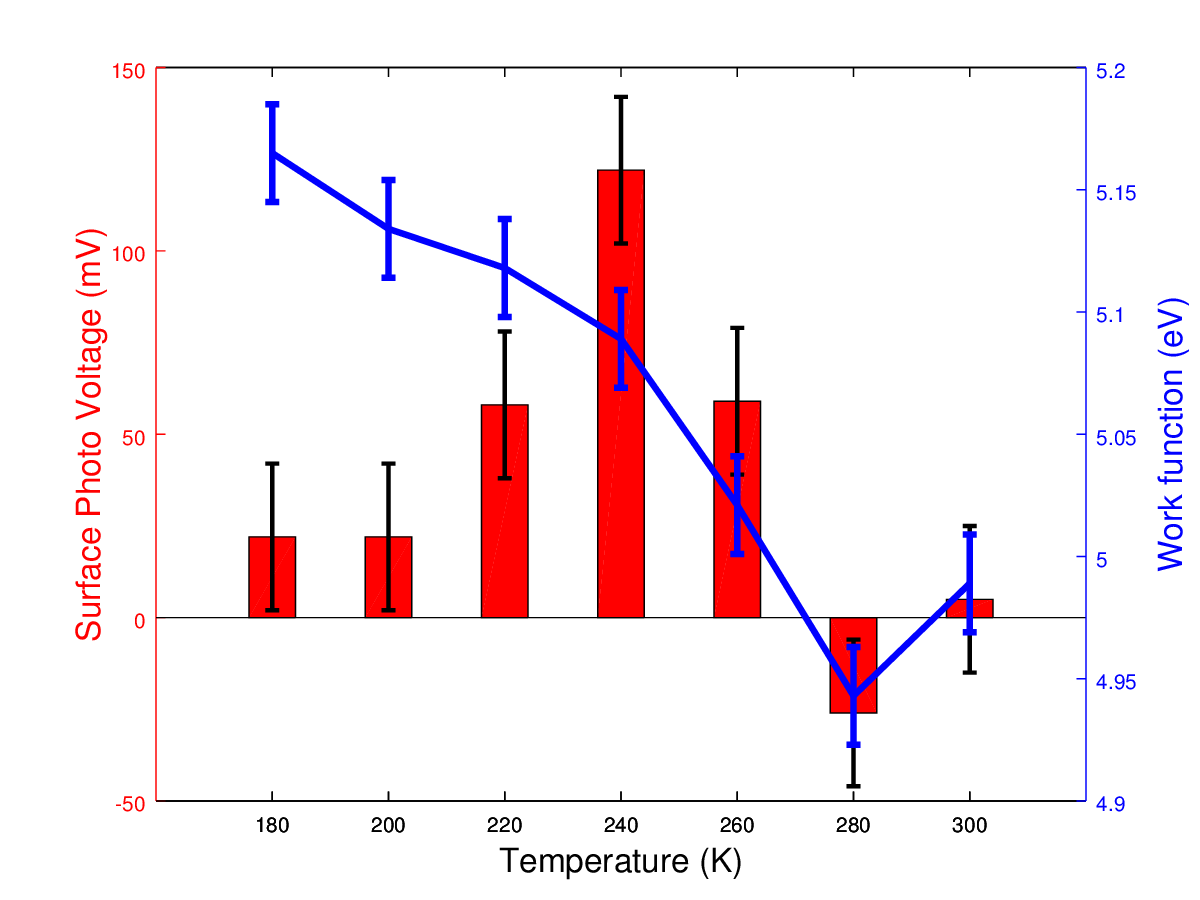
\includegraphics[width=0.8\linewidth]{./figs/chap2/vox3}
	\caption{Measured surface photovoltage and calculated work function for the \wvadiox{} sample as a function of temperature. The appearance of an \spv{} coincides with the \mit{} temperatures observed in earlier measurements, its positive sign indicates an n-type semiconductor. The change in \wf{} is substantial but remains unexplained without further experiments. Experimental uncertainties are explained in the text.}
	\label{fig:vox3}
\end{figure}
We will now concentrate on the measurement of the \spv{} as shown in Figure \ref{fig:vox3}. A significant \spv{} is observed below \SI{280}{\kelvin}, at \SI{240}{\kelvin} the \spv{} is at its maximum of $\sim$ \SI{120}{\milli\volt} and below \SI{220}{\kelvin}, the \spv{} is reduced back to levels comparable to those at room temperature. A significant \spv{} signal is therefore observed in the same temperature range that was identified for the \mit{} in the resistivity measurements. In the metallic rutile configuration, no \spv{} is observed and none is expected. As the energy gap of the material gradually widens, the \spv{} gradually increases because gradually less thermally free carriers can shield trapped surface charges in the dark condition. The simultaneous presence of both phases of vanadium-dioxide over a range of temperatures has been observed in the literature~\cite{pergament_mixphase}. As a result, band bending and hence observed \spv{} gradually increase. If the \spv{} is assumed to be saturated at \SI{240}{\kelvin} and, accordingly, the bands to be flattened, the band bending is $\sim$ \SI{120}{\milli\electronvolt}. Possible Fermi level pinning would add to the size of the band bending, so the stated value has to be seen as a minimum. On first sight, the gradual decrease in \spv{} signal might be puzzling. One would expect the trend for the \spv{} to continue, after all, the idea behind low temperature \spv{} is to counteract thermally free carriers and increase the influence of electron-hole pairs created by absorption of light. However, the observation made here can be explained if one recalls that vanadium-dioxide is undergoing a metal to \emph{insulator} transition and that for an insulator, the energy gap is expected to be relatively large. Looking at the spectrum of illumination, Figure \ref{fig:ledspec}, a clear cut off below \SI{400}{\nano\metre} is seen. \SI{400}{\nano\metre} radiation corresponds to a photon energy of $\sim$ \SI{3.1}{\electronvolt} so if the energy gap in \vadiox{} becomes larger than this, no carriers can be created by illumination or rather: only a minute fraction of incident photons corresponding to the minute fraction of photons at the low-wavelength tail of the \led{} will have sufficient energy to create free carriers. Therefore, the sample is no longer saturated by illumination and a significant drop in observed \spv{} signal is expected. A problem with that interpretation is that the band gap of vanadium-dioxide is consistently reported as $\sim$\SI{0.7}{\electronvolt}, from theoretical~\cite{biermann_theogap} as well as from experimental studies~\cite{garcia_expgap,jensen_expgap,koethe_expstud,merenda_expgap}.\\
Concentrating on the temperature range 180 to 300 K, a change in \wf{} of $\sim$ \SI{150}{\milli\electronvolt} is seen in both in Figure \ref{fig:vox2} and, more clearly, in Figure \ref{fig:vox3}. So far, positive changes of \wf{} of up to \SI{450}{\milli\electronvolt} have been observed for bundle-like \vadiox{} nanostructures~\cite{yin_450change}. A decrease of $\sim$ \SI{150}{\milli\electronvolt} was also reported by Ko~\cite{ko_kp} during the \mit{} of pure vanadium-dioxide, in contrast to the increase in \wf{} observed here for the tungsten-doped material. Tungsten should act as an n-type dopant and this is in accordance with the sign of \spv{} observed in Figure \ref{fig:vox3}. The change in \wf{} can not be explained by a gradual change in the position of the Fermi level: for an n-type material, $E_f$ is expected to increase with lowering temperature. The carrier concentrations inside the material might change drastically due to dopant freeze-out or other mechanism and that might change $E_f$ sufficiently to account for the rise in \wf{}, but without further experiments, these attempted explanations remain speculative. Judging from the reported the complexity of the electronic band structure of \vadiox{}~\cite{eyert_theobands,booth_theobands}, attempts at explaining the observed data in terms of simple band diagram considerations will fall short. Similar experiments with an extended spectral range or a more detailed study of spectral surface photovoltage might serve to explain further the results obtained for this material here, but they are out of scope of this project. Vanadium-dioxide was, above all, chosen as a system to show a viable \spv{}(T) measurement and to serve as proof of concept for the experimental system, \ie{} the combination of as Lakeshore cryogenic system coupled with a \McA{} Kelvin probe and \led{} illumination. This was achieved with these experiments.
\newpage
\section{Conclusion}
A series of experiments showed the viability of using the Lakeshore cryogenic system equipped with a \McA{} Kelvin probe head and an \led{} illumination source as a system to measure temperature dependent changes in the surface photovoltage. To do so, the \cpd{} obtained under various circumstances, namely in ambient, under low pressure and at temperatures below freezing was compared to existing, trusted systems and any deviations between the experimental systems were within experimental uncertainty. The work function of \wvadiox{} obtained from the new system also corresponded remarkably well to results reported in the literature. The \spv{} obtained from measurements in the Lakeshore at room temperature was shown to systematically be $\sim$\SI{12}{\percent} lower than the \spv{} measured with the established systems, which can be explained by unavoidable shadowing of the sample surface due to the placement of the probe-arm above and close to the sample. The temperature range for the metal-insulator transition of \wvadiox{} obtained in earlier, preliminary research carried out in the Cahen group and that reported in the literature agrees perfectly with that obtained from the appearance of an \spv{}-signal in the \spv{}(T) measurement. The precise reasons for the observed decrease of the \spv{} at temperatures below \SI{240}{\kelvin} and the drastic change in \wf{} around $\sim$\SIlist{120;170}{\kelvin} remain elusive but might be explored further with research involving expanded spectral ranges of illumination, \sps{}(T) measurements or systematic investigations of a greater variety of \vadiox{} samples. However, the practical viability of the new experimental system could still be shown with the experiments carried out during this project.


